\section{Modeling of Semi-trailer Tank Truck}
This section begins with the vehicle and liquid sloshing modeling for the MPC controller. The process of model parameter identification is then described. 

\vspace{-0.3cm}

\subsection{Semi-trailer Tank Truck Modeling}

This study focuses on semi-trailer tank trucks with higher ownership, higher load capacity, and greater susceptibility to rollover accidents. Based on a 5-degree-of-freedom(DOF) semi-trailer model \cite{ParamDisting1}\cite{ParamDisting2} and a linearized pendulum model, the semi-trailer is modeled as a 6DOF dynamic system and linearized at the current state point to support real-time calculation with certain accuracy. The coordinate definition, single pendulum dynamic model, and simplified dynamic model of the liquid tank truck are shown in Fig. \ref{fig:system_description}.

For real-time computation, a single pendulum (SP) model is used to predict liquid sloshing in the controller. Other models such as trammel pendulums (TP), combined trammel and single pendulum (TPSP), and dual mass TP (DMTP) are available for liquid sloshing modeling \cite{KomasaMutiDOF}. Even if the DMTP model has wider applicability and higher accuracy at medium and low liquid filling rates ($f\leq65\%$), it exhibits strong nonlinearity. Linearizing the DMTP model for model predictive control (MPC) requires re-linearization at each time step, while establishing a nonlinear MPC without linearization makes it challenging to find an approximate optimal solution within the time step. In finite domain MPC, the prediction accuracy of the model near the current moment significantly affects the solution's optimality and compliance with observation constraints. However, as the prediction timeline progresses, reductions in model accuracy have increasingly less effect on the actual control performance \cite{EbenLi_FastMPC}. The linearized pendulum model provides relatively accurate predictions in a short time domain, making it suitable for fast-solving MPC.

Previous studies focused on lateral acceleration input ($\ddot{y}$) and neglected roll movement \cite{WanYing2018, Yuzhixin2018, ZhaoWeiqiang2018}. However, in situations where a liquid tank truck cannot be salvaged, the roll angle ($\phi$) ranges from $12\degree$ to $18\degree$. The resulting roll moment significantly affects vehicle dynamics and liquid sloshing. Co-simulation verification of vehicle dynamics and CFD confirms that under extreme conditions like short distance double lane change (DLC), a controller based on a linearized pendulum model without considering the vehicle's roll angle fails to prevent rollover. To address this, this study incorporates both lateral acceleration ($\ddot{y}$) and roll angle ($\ddot{\phi}$) inputs into a nonlinear pendulum model, which is subsequently linearized. The impact of vertical acceleration on driving is relatively small and thus disregarded in this study. See Fig. \ref{fig:sp} for the representation of the SP model.

\begin{figure*}[!tb]
\vspace{-0.3cm}
  \centering
  \subfloat[]{
    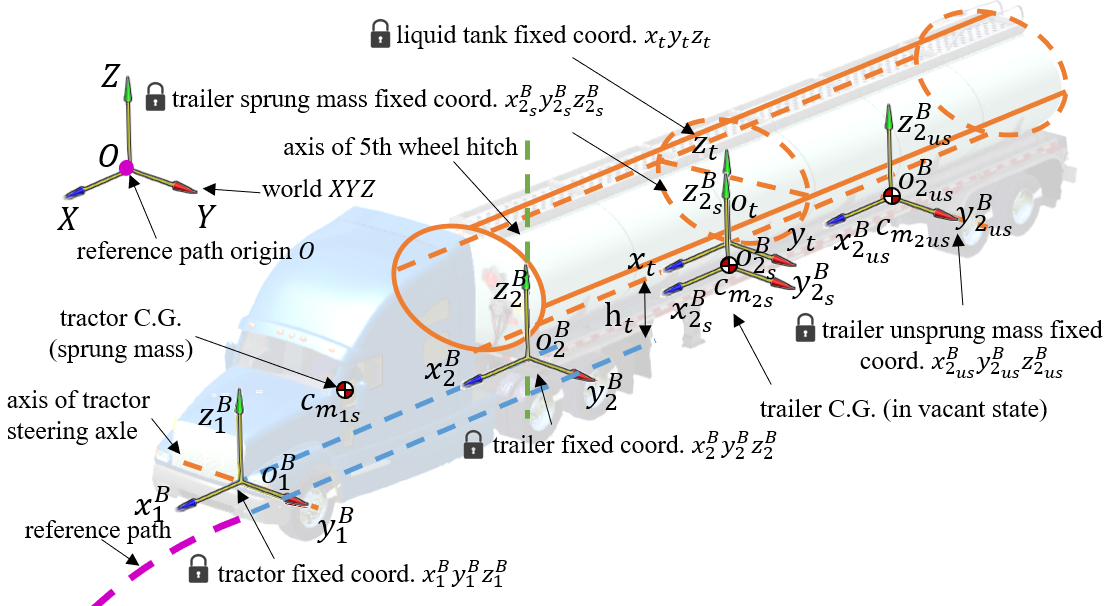
\includegraphics[width=0.5\textwidth]{fig/coordinate.png}
    \label{fig:coordinate}}
  % \hfill
  \subfloat[]{
    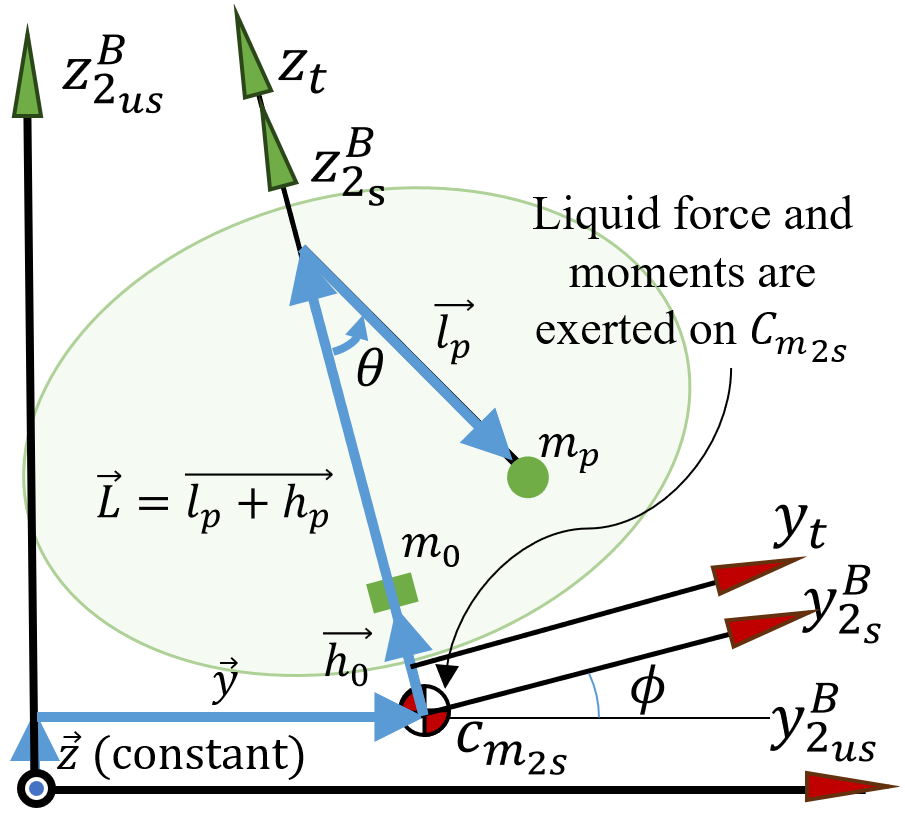
\includegraphics[width=0.26\textwidth]{fig/singlePendulum.png}
    \label{fig:sp}} 
\vspace{-0.8cm}
  
  \subfloat[]{
    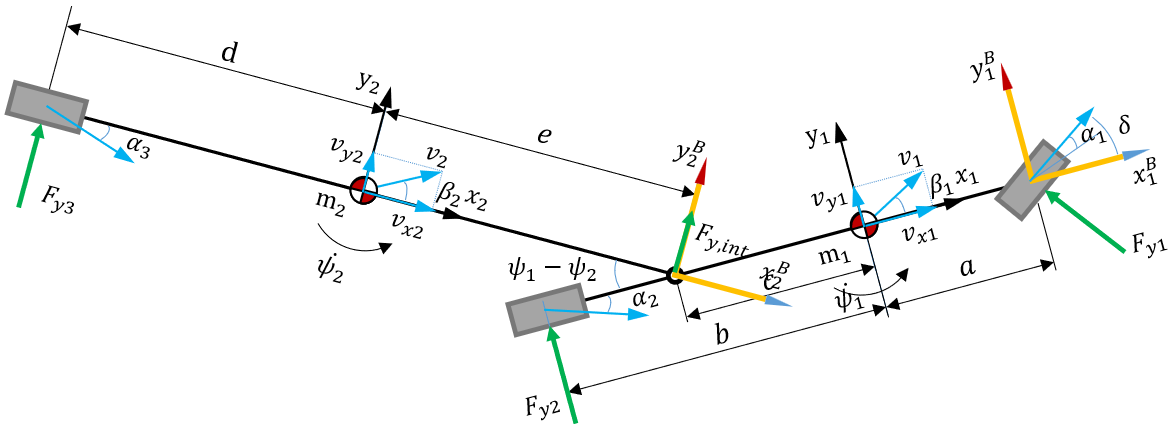
\includegraphics[width=0.60\textwidth]{fig/vehicleDynLongi.png}
    \label{fig:vehdynLongi}
  }
  \subfloat[]{
    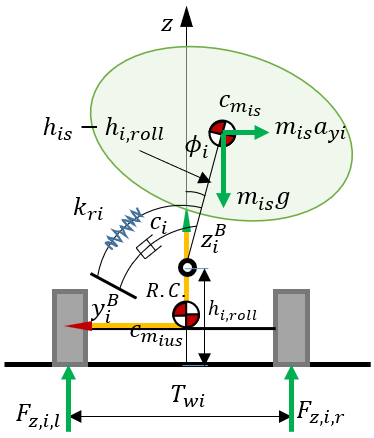
\includegraphics[width=0.20\textwidth]{fig/vehicleDynRoll.png}
    \label{fig:vehdynRoll}
  }
  \vspace{-0.2cm}
  \caption{Semi-trailer model and liquid sloshing model. (a) Coordinates definition of semi-trailer tank truck. (b) Single pendulum liquid sloshing model considering $\ddot{y}$, $\ddot{\phi}$ input, where $\phi$ is roll angle, $m_0$ and $m_p$ are static and swing mass respectively, $\theta$ is swing angle, $\vec{L}$, $\vec{l}_p$, $\vec{h}_0$, and $\vec{y}$ are geometry of pendulum. (c) Simplified semi-trailer dynamic model, parameter definition in Table.\ref{tab:parameters}. (d) Simplified semi-trailer model, depicts the roll motion around roll center (R.C.), where $g$ is gravitational acceleration.}
  \vspace{-0.8cm}
  \label{fig:system_description}
\end{figure*}


To represent the two parts of the liquid, one remains stationary and the other contributes to sloshing, two concentrated masses, $m_0$ and $m_p$, are introduced. By taking the time derivatives and second derivatives of their position vectors $\vec{R_{p0}}$ and $\Vec{R_p}$, the velocity vectors $\dot{\vec{R_{p0}}}$, $\dot{\vec{R_{p}}}$, and acceleration vectors $\ddot{\vec{R_{p0}}}$, $\ddot{\vec{R_{p}}}$ can be obtained. The system's kinetic energy $T$ and potential energy $U$ can then be expressed. By applying the Lagrange equations, the dynamic differential equation for the swinging DOF $\theta$ is derived as follows. For a detailed derivation process, please refer to technical report on \cite{CT2ROPTheoriesRepo}.

\vspace{-0.3cm}
\begin{equation}
\begin{split}
\Ddot{\theta} + \frac{1}{l_{p}}\Ddot{y}{\cos\left( {\phi + \theta} \right)} + \ddot{\phi}\left\lbrack {\left( {1 - \frac{h_{p}}{l_{p}}} \right){\cos\theta} + 1} \right\rbrack \\
- {\dot{\phi}}^{2}\left( {1 - \frac{h_{p}}{l_{p}}} \right){\sin\theta} + \frac{g}{l_{p}}{\sin\left( {\phi + \theta} \right)} + c_{d}\dot{\theta} = 0
\label{eq:lsp_dyn}
\end{split}
\end{equation}
\vspace{-0.3cm}

The derivation mentioned above is based on the assumption of no energy loss. To account for energy attenuation caused by internal flow resistance, a damping term $c_d\dot{\theta}$is added, where $c_d$ represents the damping coefficient. The lateral force and roll moment are calculated according to equations (\ref{eq:fy}) and (\ref{eq:mx}).

\vspace{-0.3cm}
\begin{equation}
F_{y} = - \left( {m_{0}\ddot{\vec{R_{p0}}} + m}_{p}\ddot{\vec{R_{p}}} \right)\vec{j}
\label{eq:fy}
\end{equation}
\vspace{-0.3cm}
\begin{equation}
\begin{split}
M_{x} = - m_{0}\left\lbrack {\vec{R_{p0}}\vec{k} \cdot \ddot{\vec{R_{p0}}}\vec{j} - \vec{R_{p0}}\vec{j}\left( {\ddot{\vec{R_{p0}}}\vec{k} + g} \right)} \right\rbrack
\\
- m_{p}\left\lbrack {\vec{R_{p}}\vec{k} \cdot \ddot{\vec{R_{p}}}\vec{j} - \vec{R_{p}}\vec{j}\left( {\ddot{\vec{R_{p}}}\vec{k} + g} \right)} \right\rbrack
\end{split}
\label{eq:mx}
\end{equation}
\vspace{-0.3cm}

After simplification, neglecting the terms related to $\dot{\phi}^2$ which are numerically small and assuming that the vehicle roll angle $\phi$ is smaller compared to the sloshing angle $\theta$, the simplified result is as follows.

\vspace{-0.5cm}
\begin{equation}
F_y = \left( m_p + m_0 \right) \ddot{y} - \left( m_0 h_0 + m_p h_p \right) \ddot{\phi} + m_p l_p \ddot{\theta}
\label{eq:fy_simple}
\end{equation}
\vspace{-0.3cm}
\begin{equation}
\begin{split}
M_x &= \left( m_0 h_0 + m_p h_p \right) g \phi + \left( m_0 h_0^2 + m_p h_p^2 \right) \ddot{\phi} \\
&\quad + m_p l_p \ddot{\theta} - \left( m_0 h_0^2 + m_p h_p^2 \right) g \theta
\end{split}
\label{eq:mx_simple}
\end{equation}
\vspace{-0.3cm}

Based on Newton's equation in the body-fixed coordinate system, $\ddot{y}$ can be expressed as $\dot{(v_{y2})}+\dot{(\phi_2)}v_{x2}$, which is $\dot{\beta}^2 + \dot{\psi}^2 = v_x^2$. Therefore, according to equations (\ref{eq:fy_simple}) and (\ref{eq:mx_simple}), the effect of liquid sloshing on the semi-trailer is incorporated into the vehicle dynamics.

As shown in Fig.(\ref{fig:vehdynLongi})(\ref{fig:vehdynRoll}), force analysis is conducted on the simplified tank truck model.

Tractor's lateral transitional, yaw, and roll motion:
\vspace{-0.3cm}
\begin{equation}
m_1 v_{1x} (\dot{\beta}_1 + \dot{\psi}_1) - m_1 s_1 h_1 \ddot{\phi}_1 = F_{y1} + F_{y2} + F_{y, int}
\end{equation}
\vspace{-10pt}
\begin{equation}
I_{1zz} \ddot{\psi}_1 - I_{1xz} \ddot{\phi}_1 = F_{y1} a \cos(\delta) - F_{y2} b - F_{y, int} c
\end{equation}
\vspace{-10pt}
\begin{equation}
\begin{split}
[I_{1xx} + m_{1s} h_1^2] \ddot{\phi}_1 - I_{1xz} \ddot{\psi}_1 = m_1 g h_1 \sin(\phi_1) \\
 + m_{1s} h_1 [\dot{v}_{1x} (\dot{\beta}_1 + \dot{\psi}_1) - h_1 \ddot{\phi}_1]
\end{split}
\end{equation}
\vspace{-0.3cm}

Trailer's lateral transition, yaw, and roll motion:

\begin{equation}
\begin{split}
m_2 v_{2x} (\dot{\beta}_2 + \dot{\psi}_2) - m_{2s} h_2 \ddot{\phi}_2 \\= F_{y3} - F_{y, int} \cos(\psi_1 - \psi_2) + F_y 
\end{split}
\end{equation}
\vspace{-10pt}
\begin{equation}
I_{2zz} \ddot{\psi}_2 - I_{2xz} \ddot{\phi}_2 = - F_{y3} d - F_{y, int} e \cos(\psi_1 - \psi_2)
\end{equation}
\vspace{-10pt}
\begin{equation}
\begin{split}
[I_{2xx} + m_{2s} h_2^2] \ddot{\phi}_2 - I_{2xz} \ddot{\psi}_2 = -m_2 g h_2 \sin(\phi_2) \\
 + m_{2s} h_2 [\dot{v}_{2x} (\dot{\beta}_2 + \dot{\psi}_2) - h_2 \ddot{\phi}_2] \\
- k_{r2} \phi_2 - c_2 \dot{\phi}_2 - k_{12} (\phi_2 - \phi_1) + F_{y3} h_{2c} + M_x 
\end{split}
\end{equation}
% \vspace{-0.6cm}


\begin{table}[!htbp]
  \centering
  \caption{Parameters and Variables}
  \label{tab:parameters}
  \begin{tabularx}{0.45\textwidth}{@{}lX@{}}
    \toprule
    \textbf{Parameter} & \textbf{Description (i=1,2 for tractor, trailer)} \\
    \midrule
    $m_i$, $m_{si}$ & Total mass of the vehicle, sprung mass \\
    $v_{ix}$, $v_{iy}$ & Longitudinal/lateral velocity \\
    $\dot{\beta_i}$ & Lateral slip angle of the center of mass \\
    $\psi_i$, $\phi_i$ & Yaw angle, roll angle \\
    $h_i$ & Distance from the center of mass to the roll center \\
    $h_{ic}$ & Height from the fifth wheel to the roll axis \\
    $I_{izz}$, $I_{ixx}$, $I_{1xz}$ & Moments of inertia for the sprung mass in yaw, roll, and cross-coupling directions \\
    $k_{ri}$,$c_i$ & Suspension roll stiffness/damping \\
    $F_{y1}$, $F_{y2}$, $F_{y3}$ & Lateral forces on the equivalent front and rear axles of the tractor, and equivalent rear axle of trailer \\
    $F_z$ & Vertical force exerted on wheels\\
    $F_{y,int}$ & Lateral force exerted by the trailer on the tractor \\
    $F_y$, $M_x$ & Liquid sloshing lateral force and roll moment\\
    $a$, $b$, $c$& Distances from the tractor's front axle/rear axle/fifth wheel hinge to the center of mass \\
    $d$, $e$ & Distance from the trailer's rear axle/fifth wheel hinge to the center of mass \\
    $k_{12}$ & Roll stiffness of the fifth wheel connection\\
    $k_1$, $k_2$, $k_3$ & Equivalent front axle, rear axle of the tractor, and trailer rear axle lateral stiffness  \\
    $\theta$ & Liquid sloshing angle \\
    $\delta$, $\delta_d$ & Steering angle, desired steering angle \\
    \bottomrule
  \end{tabularx}
\end{table}
% \vspace{-0.3cm}

The kinematic constraint equations for tractor and trailer are
% \vspace{-0.3cm}
\begin{equation}
\begin{split}
\dot{\beta}_1 - \dot{\beta}_2 - \frac{h_{1c}}{v_{1x}} \ddot{\phi}_1 + \frac{h_{2c}}{v_{2x}} \ddot{\phi}_2 - \frac{c}{v_{1x}} \ddot{\psi}_1 - \frac{e}{v_{2x}} \ddot{\psi}_2 + \dot{\psi}_1 - \dot{\psi}_2 = 0  
\end{split}
\end{equation}

Due to the use of a linear tire model, lateral forces of each equivalent axis can be approximated as
\begin{equation}
\left\{\begin{split}
F_{y1} &= k_1 [\beta_1 + \frac{a}{v_{1x}} \dot{\psi}_1  - \delta ] \\
F_{y2} &= k_2 [\beta_1 - \frac{b}{v_{1x}} \dot{\psi}_1] \\
F_{y3} &= k_3 [\beta_2 - \frac{d}{v_{2x}} \dot{\psi}_2]
\end{split}\right.
\end{equation}

where parameters are described in Table.\ref{tab:parameters}.

On the basis of the above nonlinear dynamic differential equations, linearization is performed by making the following assumptions: the hinge angle ($\psi_1-\psi_2$) is small, i.e., $\cos(\psi_1-\psi_2)\approx 1$; the roll angles of the tractor and semi-trailer are small, i.e., $\sin(\phi_i)\approx \phi_i$, where $i=1,2$; the front wheel steering angle $\delta$ is small, i.e., $\cos(\delta)\approx 1$. 

To facilitate the calculation of vehicle dynamics and sloshing models, as well as to meet the requirements for predicting the vehicle's pose state variables in path tracking, the following 14 state variables are selected to construct the state space equation. Explanation for each state variable in Table.\ref{tab:parameters}.

\vspace{-0.3cm}
\begin{equation}
X = \left[v_{1y}\,\dot{\psi}_1\,\phi_1\,\dot{\phi}_1\,\,v_{2y}\,\dot{\psi}_2\,\phi_2\,\dot{\phi}_2\,\theta\,\dot{\theta}\,\psi_1\,v_{1x}\,Y_1\,X_1\right]^T
\label{eq:xk}
\end{equation}
\vspace{-0.3cm}

Among them, $Y_1$, $X_1$ denotes the tractor's coordinates. Means of measurement in real application is described in Table.\ref{tab:measurement}
The linearized vehicle state space equation is established as follows. 

\vspace{-0.3cm}
\begin{equation}
\dot{X} = A_c X + B_c \delta
\label{eq:c_time_ss_model}
\end{equation}
\vspace{-0.3cm}

Matrices $A_c$ and $B_c$ are defined in Appendix A\ref{appendix:A}. Steering actuator dynamics can diverge the controller if its time constant is large, and compensation can be made by converting the steering angle $\delta$ as a state variable, while adding the desired steering angle $\delta_{d}$ as a manipulated variable, constructing a new state space as

\vspace{-0.3cm}
\begin{equation}
\begin{bmatrix} \dot{X} \\\dot{\delta}  \\\end{bmatrix} = \begin{bmatrix} 
  A_c & B_c\\
  0   & -1/\tau_{s} \\
\end{bmatrix}\begin{bmatrix} X \\\delta  \\\end{bmatrix}
+\begin{bmatrix} \textbf{0} \\1/\tau_{s}  \\\end{bmatrix}\delta_{d}
\label{eq:steerActuator_ss_model}
\end{equation}
\vspace{-0.3cm}

where $\tau_s$ is the steering actuator time constant. After testing, it was found that when the steering dynamics are modeled as an inertia system with appropriate compensation in the controller, the tracking performance is not significantly affected. Therefore, for the sake of simplicity, steering dynamics are neglected in the following simulations and model experiments. However, they must be fully considered in the implementation of a full-size vehicle.

When solving, perform zero-order hold discretization on the state-space equation, i.e.

\vspace{-0.3cm}
\begin{equation}
X_k = A_d X_{k-1} + B_d \delta_k
\end{equation}

Where $k$ represents the $k$-th time step, the discretized state transition matrix $A$ and input matrix $B$ are obtained as follows.

\vspace{-0.3cm}
\begin{equation}
\begin{bmatrix}
A_{d} & B_{d} \\
\bold{0}_{N_{u} \times N_{x}} & \bold{I}_{N_{u}}
\end{bmatrix} = {{\exp m}\left( {T_{s}\begin{bmatrix}
A_{c} & B_{c} \\
\bold{0}_{N_{u} \times N_{x}} & \bold{0}_{N_{u}}
\end{bmatrix}} \right)}
\label{eq:system_discrete}
\end{equation}


Here, $T_s$ is the time step of the discretized model, $\text{expm}(\cdot)$ is the matrix exponential function, $n_x$ and $n_u$ represent the number of state variables and control variables in the model, respectively. For equation (\ref{eq:system_discrete}), we have $ N_x=14$ and $N_u=1$. The discrete state transition matrix $A$ and input matrix $B$ are calculated by substituting the current values of $v_{1x}$ and $v_{2x}$ into the equations. At each time step, matrix $A$ and $B$ are recalculated to form a linear time-varying model.





















\vspace{-0.5cm}
\subsection{Parameter identification}
The cross-section geometry of the tank used for simulation in this research is illustrated in Fig.(\ref{fig:tank_geo}), which has an overall elliptical shape with the length of 11 meters and is divided into 8 homogeneous compartments by wave-proof plates with alternating directional holes on both the middle and bottom.


\begin{figure}[!htb]
\centering
\vspace{-0.3cm}
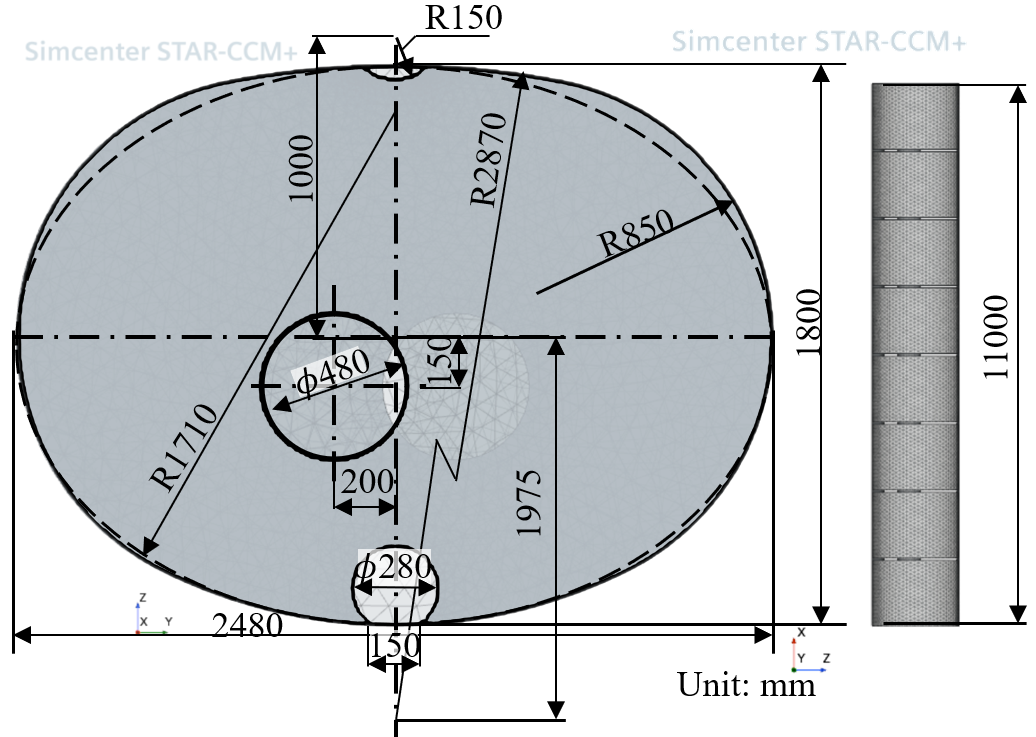
\includegraphics[width=2.5in]{fig/tank_geometry.png}
\vspace{-0.3cm}
\caption{Tank cross-section geometry used in simulation.}
\vspace{-0.3cm}
\label{fig:tank_geo}
\end{figure}


Parameter identification of the linearized SP model can be achieved through calibration using CFD simulation results as true values. Establish CFD simulations under standard lateral acceleration step excitation conditions that cover most of the actual driving condition parameter ranges, as shown in Fig. \ref{fig:dataset}. The most dangerous filling rate $f=50\%$ is chosen to test the worst case.

\begin{figure}[!htb]
\centering
\vspace{-0.4cm}
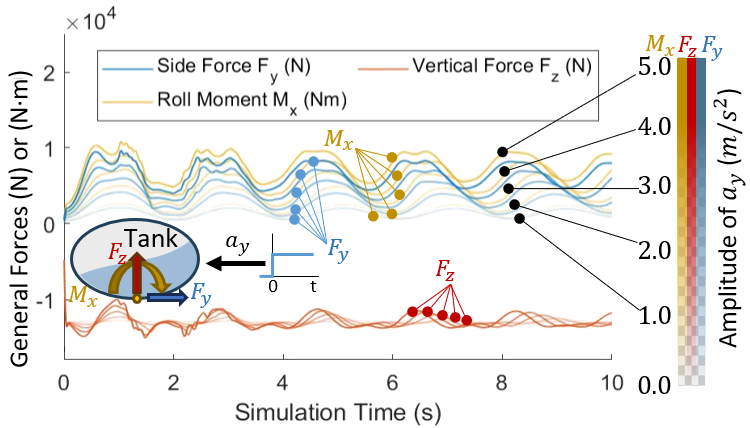
\includegraphics[width=3.5in]{fig/stepDataset.png}
\vspace{-0.6cm}
\caption{CFD simulation dataset showing the side force $F_y$, vertical force $F_z$, and roll moment $M_z$ over time with step excitation of lateral acceleration $a_y(t)=Const$, $Const=1,2,3,4,5m/s^2$, filling rate $f=50\%$.}
\vspace{-0.3cm}
\label{fig:dataset}
\end{figure}

Pendulum tend to follow input frequency during forced sloshing. Conversely, the model differences become more pronounced under free sloshing due to differences in natural frequencies. To address this, a lateral acceleration step excitation dataset is established and used for parameter identification, by applying the same lateral acceleration input from the CFD dataset to the model. By this means, the resultant acceleration of gravity and newly exerted lateral acceleration could be regarded as a new tilted synthesized gravity, creating free sloshing behavior. A mean squared deviation cost function is constructed based on the normalized three-dimensional force $F_y$, $F_z$, $M_x$, of the CFD dataset.



On the basis of the above cost, considering the trend of the free sloshing frequency increasing with the lateral acceleration amplitude of the system input as shown in Fig. \ref{fig:dataset}, the SP model parameters fitted with a specific lateral acceleration (e.g. $a_y=3m/s^2$) as the standard operating condition have significant phase errors under other acceleration values, resulting in over-fitting of the parameters. Therefore, the non-negative weighted sum of the mean squared deviation of the three-dimensional force under 5 working conditions $a_y=1,2,3,4,5m/s^2$ is used to construct the cost function as shown in equation (\ref{eq:fitting}).

\vspace{-0.3cm}
\begin{equation}
\begin{split}
J &= \left\| \frac{{F_{y,a_y} - F_{y,0,a_y}}}{\bar{F_{y_0,a_y}}} \right\|^2 + w_2 \left\| \frac{{F_{z,a_y} - F_{z,0,a_y}}}{\bar{F_{z_0,a_y}}} \right\|^2 \\
&+ w_3 \left\| \frac{{M_{x,a_y} - M_{x,0,a_y}}}{\bar{M_{x_0,a_y}}} \right\|^2, \quad a_y = 1,2,3,4,5 
\label{eq:fitting}
\end{split}
\end{equation}
\vspace{-0.3cm}

\begin{figure}[!htb]
\centering
\vspace{-0.2cm}
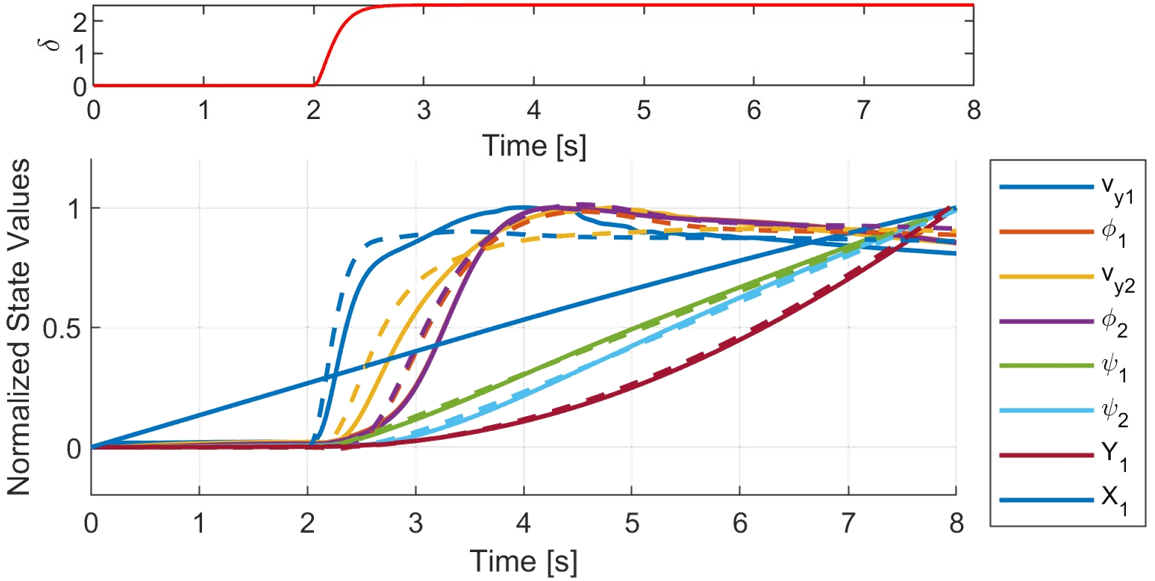
\includegraphics[width=3.5in]{fig/6DOF_exp.png}
\vspace{-0.6cm}
\caption{Fitting results under steering angle $\delta$ step 2.5$\degree$ condition, 65 km/h, filling rate $f=50\%$. Dashed lines are from linear model, and solid lines are from TruckSim model.}
\vspace{-0.3cm}
\label{fig:6dof_exp}
\end{figure}

\vspace{-10pt}
\begin{table}[!htbp]
  \centering
  \caption{Linearized SP Parameters identification Results}
  \label{tab:pararecog}
  \begin{tabularx}{0.45\textwidth}{lp{3.5cm}lp{8.5cm}l@{}l}
    \toprule
    \textbf{Symbol} & \textbf{Parameter Description} & \textbf{Values ($f=50\%$)} \\
    \midrule
    $m_p$ & Swing mass $m=m_p+m_0$ & 11660 [kg] \\
    $h_0$ & Relative height of $m_0$ to tank bottom & 1.161 [m] \\
    $h_p$ & Minimum relative height of $m_p$ to tank bottom & 0.255 [m] \\
    $l_o$ & Length of pendulum & 0.981 [m] \\
    $c_d$ & Swinging damping & 0.1345 [null] \\
    \bottomrule
  \end{tabularx}
\end{table}
\vspace{-0.3cm}

The normalized mean values of the three-dimensional forces in the CFD step dataset, $\bar{F_{{y0},a_y}}$, $\bar{F_{{z0},a_y}}$, and $\bar{M_{{x0},a_y}}$, are calculated. The weighting coefficients $w_i \geq 0$, where $i=1,2,3$, are applied. $F_{y,a_y}$ represents the lateral force output of the model under a step excitation of lateral acceleration $a_y$. $F_{z,a_y}$ represents the vertical force output of the model under a step excitation of lateral acceleration $a_y$. $M_{x,a_y}$ represents the roll moment output of the model under a step excitation of lateral acceleration $a_y$. All three force outputs are in the form of time sequences, denoted as $k$ representing the output at the $k$-th time step, with a total of $N+1$ time steps.

Using genetic algorithm to optimize the cost function above to obtain the equivalent pendulum model parameters, the physical meanings of each parameter and the identification results at 50\% liquid filling rate are shown in Table.\ref{tab:pararecog}, where $m$ is the total liquid mass, $m=14462 kg$ when $f=50\%$.

The steering angle step condition is used to assess the model's accuracy, as illustrated in Fig.\ref{fig:6dof_exp}. Key state variables are normalized to present the fitting results between the 6DOF semi-trailer tank truck linear model and the high-fidelity TruckSim simulation results.














